%!TEX root = ../proposal.tex
\section{Introduction and Motivation}
Self-Driving Cars are becoming one of the most profound technologies and the Auto Makers compete for the dominance of the technology\cite{hancock2019future}. Autonomous cars are becoming more intelligent and expected to replace the human drivers and increase the safety of roads by avoiding traffic accidents. The sales of autonomous cars is expected to reach 90\$ Billion in 2030\cite{bertoncello2015ten}\cite{keeney2017mobility}.There are several ongoing projects within this domain (e.g. Waymo \cite{teoh2017rage}), most of them are advance enough to deploy on roads and under testing in everyday life. However, the development of fatal crashes in autonomous cars raises questions about the testing of controlling software and decision making in critical scenarios \cite{zhou2017identification}. The testing of autonomous cars on public road is necessary for the development and enhancement of self driving technology because autonomous cars does not know how to behave with the unfamiliar situation or scenarios. Testing of the autonomous cars on real road for number of days to find the flaws is time consuming and tremendously challenging task. 


The traditional way of testing the self-driving cars for naturalistic driving scenarios is Field Operational Tests (FOT). The downside of FOT that it won't be able to cover all the interesting scenarios and need to cover million of miles to test erroneous behavior and damage (failure) because of collision with car, pedestrian etc \cite{kalra2016driving}. The relevant instance of autonomous car crashes are Waymo, Uber and Tesla Car crash. The Uber self-driving car \cite{levin2018uber} \cite{kohli2019enabling} failed to recognize an object such as women
which caused it to ignore a pedestrian walking and classified as "false positives," that wouldn't be an issue for the vehicle, like a plastic bag or piece of paper. On the other side, Google self-driving car \cite{muir2016google} hit the bus while changing the lane on the series of assumption of Google's program. The car anticipated that the bus will allow slow down and allow the car to cut in. Hence, it shows that the self-driving car are far away from handling the critical scenarios and sustainable testing system is required for the testing of autonomous cars to prevent the accidents and enhance the safety of roads and society. 

Another possibility of testing autonomous cars is the virtual testing, where the car controlling software \cite{zhang2014roadview} is simulated with different testing parameters and environmental conditions \cite{tian2018deeptest}\cite{ben2016testing}. The distinct input in the self-driving cars with realistic scenarios in virtual testing will reduce the cost of physical testing. Indeed, the virtual testing can't replace the real world testing but it narrow the gap in the testing of autonomous cars \cite{sippl2016simulation}. 

The NHTSA (National Highway Traffic Safety Administration) \cite{stocker2019shared} formulated to save lives, increase safety, and reduce the autonomous car crashes through research and enforcement activity. The administration of NHTSA is enforcing the safety equipment in motor vehicles and emerging Automated Driving System (ADS). However, the Automotive industry does not established any rules and regulation to certify autonomous cars. Therefore, NHTSA has a formed a regulative body for the evaluation of new technologies and test the self-driving cars in critical scenarios before the deployment on public roads. The accidental crash report on NHTSA database does not provide any information about the car velocity, acceleration and steering angle. The crash report is semi-structured to unstructured multimedia documents with the description of the precrash event, collision impact of the cars and after crash event, the speed limit of the vehicles on specific road and written in natural language. The non-trivial problem in unstructured data extract meaningful information for faster decision-making.

The safety of the autonomous car unknown at design time and safe motion plan is highly unpredictable in complex or critical scenarios. It is hard to try all the possible environments in autonomous driving and autonomous vehicles will encounter the situation that have not been tested before\cite{althoff2018automatic}. The velocity of the car highly impact the drivable area of each vehicle and time to reach the target point. The autonomous vehicles is look forward to adapt the velocity according to the environment and drive smoothly without any external output\cite{altche2017high}. However, many of the existing autonomous cars are incapable of making such adjustment. The autonomous car drive on the assumption that feasible velocity reference is given and predetermined path of autonomous car and surrounding car are not going to collide with each other on given speed. Moreover, the speed limit on lanes, highways make the trajectory planning high complex and computation difficult. To address this problem, the parameter space of velocity will be explored for the crash scenario and the mutant parameter that does not effect the outcome of the crash. The range of velocity at certain scenario will help the autonomous car to make the adjustment in the speed with the other traffic participants. 

In this thesis, the motive is to perform parameter exploration such as velocity, acceleration to estimate the speed of the car crash during collision.  The system will apply Natural language Processing (NLP) and Ontology concepts to extract the key features from semi-structured to unstructured crash reports about the vehicle, environment, car dynamics and generate the configuration file. The configuration file will be used to generate test cases to explore parameters and to reproduce the original simulation with different numerical values. The accuracy of the original and derived simulation from BeamNG\cite{beamng_research} will be evaluated from the Structured Similarity Index Matching (SSIM) and Mean Square Error (mse) computed on trajectory path after the impact/accident of car. After the series of simulation, the Decision Tree will be generated to select the best parameters (Test Case) that reflect the original simulation. It will help to identify the search of requirement for the speed of autonomous cases, violations and worst cases. The parameter is only restricted to two dimensions because focusing on the combinatorial coverage of more than 2 dimensions is impractical.

\subsection{Research Questions}
This thesis will look into the following research questions:

\begin{itemize}
  \item	Explore the missing parameters such as velocity, steering angle in the crash report.
  \item	Identify the list of possible parameters and their values that produce the same critical scenario.
  \item	How can we choose the best parameters from the Decision Tree with low error. 
\end{itemize}

\begin{figure}[H]
\centering
  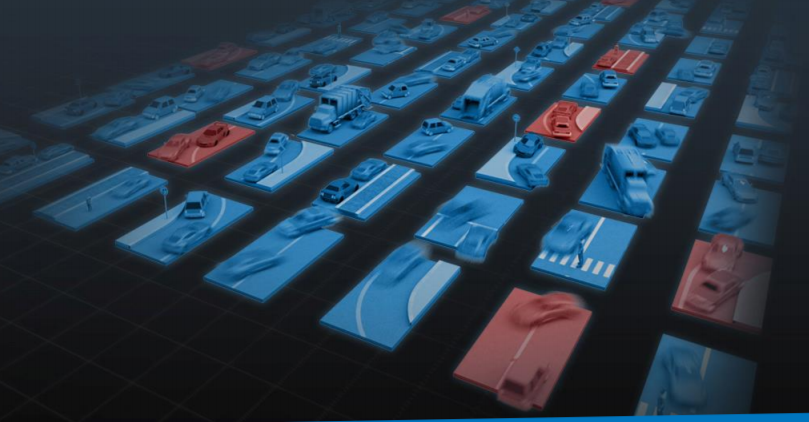
\includegraphics[scale= 0.4]{pictures/CrashScenarios.png}
  \caption{}
\end{figure}

\subsection{Improvement}
Relaxing the assumptions on crash reports and their structure by devising a better, more general, NLP information extraction. At the moment, AC3R assumes that the 1st paragraph of the police report lists only environmental elements, and the 2nd the development of the crash.

\subsection{Problem Statement}

Our aim of the research is to explore the missing parameters of the velocity and steering angle to simulate the critical crash of the autonomous vehicles as close to the description of the accident in the crash report. The relaxation on the structure assumptions of semi-structured to unstructured text in crash to devise better natural language information extraction. 


The velocity and steering angle parameter of the collision is difficult to address the parameter space becomes huge when considering the velocity and steering angle of both ego car and victim car. The autonomous cars drive on the assumption that feasible velocity reference is given and predetermined path of autonomous car and surrounding car are not going to collide with each other on given speed. The information extraction becomes complex in the case that each word context and it relationship with other sentences has to analyzed before extracting the key feature. 



